\begin{figure}[H]
\centering
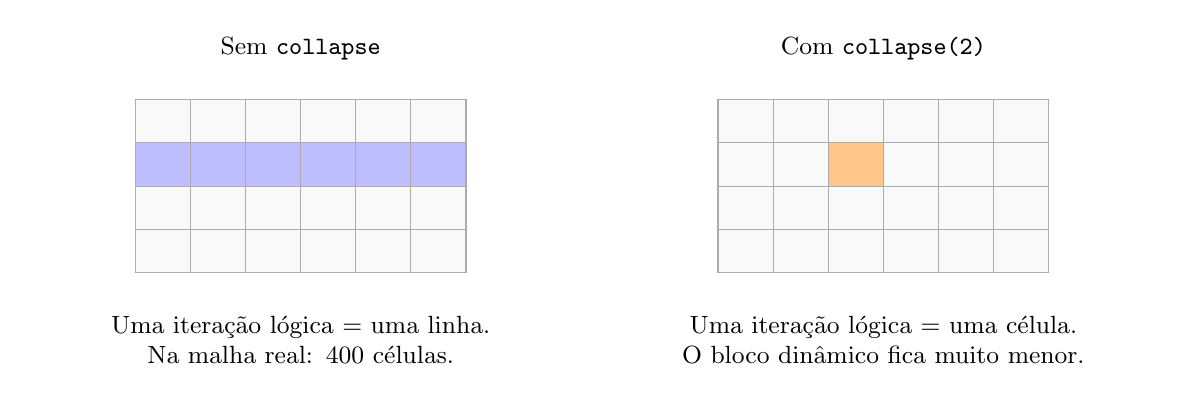
\begin{tikzpicture}[font=\small]
\foreach \s/\titulo in {0/{Sem \texttt{collapse}},7.4/{Com \texttt{collapse(2)}}}{
  \begin{scope}[xshift=\s cm]
  \node[align=center] at (2.1,.65) {\titulo};
  \foreach \r in {0,...,3}{
    \foreach \c in {0,...,5}{
      \fill[gray!5] (\c*.7,-\r*.55) rectangle ++(.7,-.55);
      \ifdim \s pt=0pt
        \ifnum\r=1 \fill[blue!25] (\c*.7,-\r*.55) rectangle ++(.7,-.55);\fi
      \else
        \ifnum\r=1 \ifnum\c=2 \fill[orange!45] (\c*.7,-\r*.55) rectangle ++(.7,-.55);\fi\fi
      \fi
      \draw[gray!65] (\c*.7,-\r*.55) rectangle ++(.7,-.55);
    }
  }
  \end{scope}
}
\node[align=center,text width=6.7cm] at (2.1,-3.05)
{Uma iteração lógica = uma linha.\\Na malha real: 400 células.};
\node[align=center,text width=6.7cm] at (9.5,-3.05)
{Uma iteração lógica = uma célula.\\O bloco dinâmico fica muito menor.};
\end{tikzpicture}
\caption{Unidade de distribuição ilustrada em uma malha reduzida. Com \texttt{dynamic,8}, a malha real de $400\times400$ distribui blocos de 3.200 células sem \texttt{collapse} e de oito células com \texttt{collapse(2)}.}
\label{fig:particionamento}
\end{figure}
